\iffalse
\let\negmedspace\undefined
\let\negthickspace\undefined
\documentclass[journal,12pt,onecolumn]{IEEEtran}
\usepackage{cite}
\usepackage{amsmath,amssymb,amsfonts,amsthm}
\usepackage{algorithmic}
\usepackage{graphicx}
\usepackage{textcomp}
\usepackage{xcolor}
\usepackage{txfonts}
\usepackage{listings}
\usepackage{enumitem}
\usepackage{mathtools}
\usepackage{gensymb}
\usepackage{comment}
\usepackage[breaklinks=true]{hyperref}
\usepackage{tkz-euclide} 
\usepackage{listings}
\usepackage{gvv}                                        
\def\inputGnumericTable{}                                 
\usepackage[latin1]{inputenc}                                
\usepackage{color}                                            
\usepackage{array}                                            
\usepackage{longtable}                                       
\usepackage{calc}                                             
\usepackage{multirow}                                         
\usepackage{hhline}                                           
\usepackage{ifthen}                                           
\usepackage{lscape}
\usepackage{siunitx}
\usepackage{flushend}
\usepackage[siunitx]{circuitikz}
\usepackage{caption}
\usepackage{setspace}

\newtheorem{theorem}{Theorem}[section]
\newtheorem{problem}{Problem}
\newtheorem{proposition}{Proposition}[section]
\newtheorem{lemma}{Lemma}[section]
\newtheorem{corollary}[theorem]{Corollary}
\newtheorem{example}{Example}[section]
\newtheorem{definition}[problem]{Definition}
\newcommand{\BEQA}{\begin{eqnarray}}
	\newcommand{\EEQA}{\end{eqnarray}}
\newcommand{\define}{\stackrel{\triangle}{=}}
\theoremstyle{remark}
\newtheorem{rem}{Remark}
\begin{document}
	
	\bibliographystyle{IEEEtran}
	\vspace{3cm}
	
	\title{NCERT 9.5 Q.27}
	\author{EE23BTECH11203 - Adarsh A$^{*}$% <-this % stops a space
	}
	\maketitle
	%\newpage
	\bigskip
	
	\renewcommand{\thefigure}{\theenumi}
	\renewcommand{\thetable}{\theenumi}
	
	
	\vspace{0.2cm}
	\linespread{1.1}
	%\onehalfspacing
	
	%\fontsize{14}{20}\selectfont
	\textbf{Question : }
	A farmer buys a used tractor for Rs 12000. He pays Rs 6000 in cash and agrees to pay the balance in annual installments of Rs 500 plus 12 \% interest on the unpaid amount. How much will the tractor cost him?
	
	\vspace{0.3cm}
	
	\solution
	\fi
	
	\begin{table}[htbp]
	\centering
	\noindent
	\fontsize{10}{15}\selectfont {
		\resizebox{0.75\textwidth}{!}{%
			\begin{tabular}{|c|c|c|}
				\hline
				\textbf{Parameter} & \textbf{Value} & \textbf{Description} \\
				\hline
				$n$ + 1 & - & Number of years \\
				\hline
				$a$ & 6000 & Amount paid\\
				\hline
				$r$ & 6000 & Remaining Amount\\
				\hline
				$x\brak n$ & $\brak{1220 - 60n}\hspace{0.1cm} u\brak n$ & Amount to be paid at ($n + 1$)$^{th}$ year \\
				\hline
				$y\brak n$ & $\brak{1220 + 1190n - 30n^2} \hspace{0.1cm} u\brak n$ & Total amount after $(n + 1)$ yrs \\
				\hline
			\end{tabular}
	} }
	
	\caption{Input Table}
	
\end{table}

	
	\vspace{0.2cm}
	
	
	
	Number of years taken to pay the remaining amount,
	\begin{align}
		n + 1 &= \dfrac{r}{500} \\
		n &= 11
	\end{align}
	
	The amount to be paid by the farmer after $(n+1)$ year/s is,
	\begin{align}
		x\brak n &= 500 + 0.12 \brak{6000 - 500n} \\
		x\brak n &= \brak{1220 - 60n}\hspace{0.1cm} u\brak n
	\end{align}
	
	Some results,
	\begin{align}
		x\brak n &
		\xleftarrow[]{\hspace{0.8cm}{\mathcal{Z}}\hspace{0.4cm}}\xrightarrow[]{}
		X\brak z\\[10pt]
		u\brak n &
		\xleftarrow[]{\hspace{0.8cm}{\mathcal{Z}}\hspace{0.4cm}}\xrightarrow[]{}
		\dfrac{1}{1 - z^{-1}} : U\brak z\\[10pt]
		n.u\brak n &
		\xleftarrow[]{\hspace{0.8cm}{\mathcal{Z}}\hspace{0.4cm}}\xrightarrow[]{}
		-z \hspace{0.1cm} \dfrac{d}{dz} \hspace{0.1cm} \dfrac{1}{1 - z^{-1}} = \dfrac{z^{-1}}{\brak{1 - z^{-1}}^2}
	\end{align}
	
	By taking $z$ transform,
	\begin{align}
		X\brak z &= \dfrac{1220}{1 - z^{-1}} - \dfrac{60 z^{-1}}{\brak{1 - z^{-1}}^2} \\[10pt]
		X\brak z &= \dfrac{1220 - 1280 z^{-1}}{\brak{1 - z^{-1}}^2} \hspace{0.2cm}, \hspace{0.3cm}\lvert \hspace{0.1cm} z \hspace{0.1cm}\rvert \hspace{0.1cm} \textgreater \hspace{0.1cm} 1 
	\end{align}
	
	%\vspace{0.3cm}
	
	Convolution in time domain is multiplication in $z$ domain :
	\begin{align}
		y\brak n &= x\brak n \ast u\brak n\\
		Y\brak z &= X\brak z . U\brak z\\[3pt]	
		Y\brak z &=  \dfrac{1220 - 1280 z^{-1}}{\brak{1 - z^{-1}}^2}.\dfrac{1}{1 - z^{-1}} \\[10pt]
		Y\brak z &= \dfrac{1220 - 1280 z^{-1}}{\brak{1 - z^{-1}}^3} \hspace{0.2cm}, \hspace{0.3cm}\lvert \hspace{0.1cm} z \hspace{0.1cm}\rvert \hspace{0.1cm} \textgreater \hspace{0.1cm} 1
	\end{align}
	
	%\vspace{0.2cm}
	Using Partial fractions,
	\begin{align}
		Y\brak z &= \dfrac{A z}{z-1} + \dfrac{B z}{\brak{z-1}^2} + \dfrac{C z}{\brak{z-1}^3}
	\end{align}
	\begin{align}
		A &= 1220\\
		B &= 1160\\
		C &= -60
	\end{align}
	\begin{align}
		\dfrac{n\brak{n-1}\brak{n-2}...\brak{n-k-2}}{k!} u\brak n &
		\xleftarrow[]{\hspace{0.8cm}{\mathcal{Z}}\hspace{0.4cm}}\xrightarrow[]{}
		\dfrac{z}{\brak{z - 1}^k}
	\end{align}
	%\vspace{-0.25cm}
	Using this result,
	\begin{align}
		y\brak n &= 1220 \hspace{0.1cm} u\brak n + 1160 \hspace{0.1cm} n \hspace{0.1cm} u\brak n - 60 \hspace{0.1cm} \dfrac{n\brak{n-1}}{2}\hspace{0.1cm} u\brak n \\
		y\brak n &= \brak{1220 + 1190n - 30n^2} \hspace{0.1cm} u\brak n \\
		y\brak {11} &= 10680
	\end{align}
	
	The total tractor cost to be paid,
	%\vspace{-0.2cm} 
	\begin{align}
		&= a + y\brak {11}\\
		&= 16,680
	\end{align}
	%\newpage
	
	%\underline{Plot of $y\brak n$ $vs$ $n$} :
	
	\begin{figure}[htbp]
		\centering
		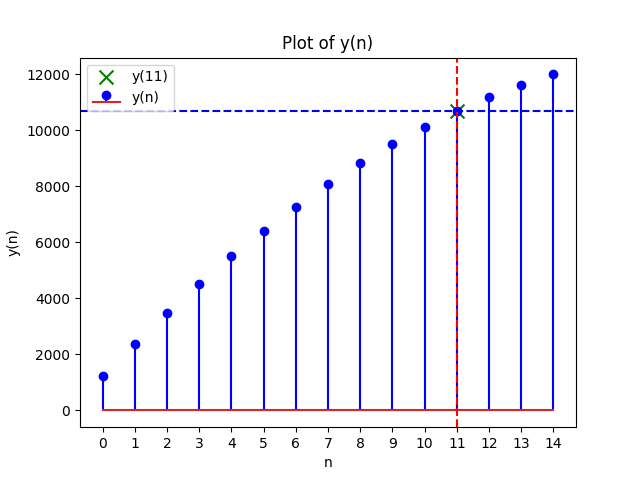
\includegraphics[width=0.6\textwidth]{ncert-maths/11/9/5/27/figures/Figure1.png}
		\caption{(a) Plot of $y\brak n$ $vs$ $n$}
		
	\end{figure}
	
%\end{document}
